\chapter{Antecedentes y estado actual}
\section{Redes neuronales}
Pese a que es ahora, en los últimos años cuando, debido a la explosión
del fenomeno de la \textit{inteligencia artificial}, comienza a ser
más popular todo lo relacionado con la dotación de inteligencia a
los dispositivos electrónicos; todo comenzó hace muchas décadas\textsuperscript{\cite{na8}}.
Ya en 1943, \textit{Warren McCulloch} (neurofisiologo) y
\textit{Walter Pitts} (matemático),
escribieron un artículo\textsuperscript{\cite{McCulloch}} acerca de las neuronas e incluso en el mismo,
fueron capaces de diseñar una red neuronal simple usando exclusivamente
circuitos eléctricos y fundamentado en algoritmos de \textit{Lógica de umbral}
(\textit{Threshold logic}).


Más tarde, en la década de 1950, en los laboratorios de \textit{IBM} de
la mano de \textit{Nathanial Rochester}, ocurrió el primer
intento de simulación de red neuronal; intento que desembocó en fracaso.
Sin embargo fue muy estimulante para el campo de la \textit{IA}
y motivó el planteamiento de lo que denominaron "máquinas pensantes".
También hubo otros acercamientos como la sugerencia del insigne
\textit{John Von Neumann} de utilizar relés telegráficos o
tubos de vacío para simular el funcionamiento simplificado de
las neuronas.


No obstante, no sería hasta 1958 que el neurobiólogo
\textit{Frank Rosenblatt} comenzaría a trabajar en el \textit{Perceptron}\textsuperscript{\cite{Rosenblatt}},
para muchos el nacimiento de la red neuronal artificial. Como todo precursor,
era simple y limitado; hoy se catalogaría de monocapa, algo que evidentemente,
ya no se usa en redes neuronales contemporaneas.
Como puede observarse en la Figura \ref{perceptron} sirviéndose de múltiples entradas binarias, era capaz de producir una
única salida, basada ya entonces en la utilización de \textit{pesos}
(número que cuantifica la relevacia de la entrada respecto de la salida),
conservada hasta día de hoy, aunque cabe destacar que entonces, los pesos
eran directamente atribuidos por el científico al cargo.
La salida binaria de esta neurona \textit{Perceptron},
sería como consecuencia de la superioridad o la inferioridad de la
suma de la multiplicación de los pesos respecto de un umbral; es por esto
que es sabida su influencia del trabajo de \textit{Warren McCulloch} y
\textit{Walter Pitts} anteriormente mencionado. Por tanto se podía destinar
a funciones lógicas binarias simples (OR/AND).


El siguiente paso natural era aumentar el número neuronas y capas,
llegando en 1965 el \textit{Multilayer Perceptron}
\textit{Perceptron}\textsuperscript{\cite{mlperceptron}}. Como consecuencia
de esta mejora y aumento de la complejidad, nacieron los conceptos de
capas de entrada, ocultas y de salida, tal y como se puede observar en la
Figura \ref{MLPerceptron}. De igual forma y dado que el
reparto de pesos todavía no se había automatizado, los valores con los
que se trabajaban, seguían siendo binarios.

\begin{figure}[h]
    \centering
    \subfloat[Perceptron\label{perceptron}]{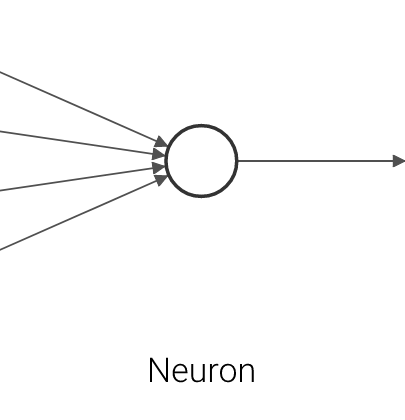
\includegraphics[width=0.25\textwidth]{capturas/esquemaPerceptron.png}}
    \hfill
    \subfloat[Multilayer Perceptron\label{MLPerceptron}]{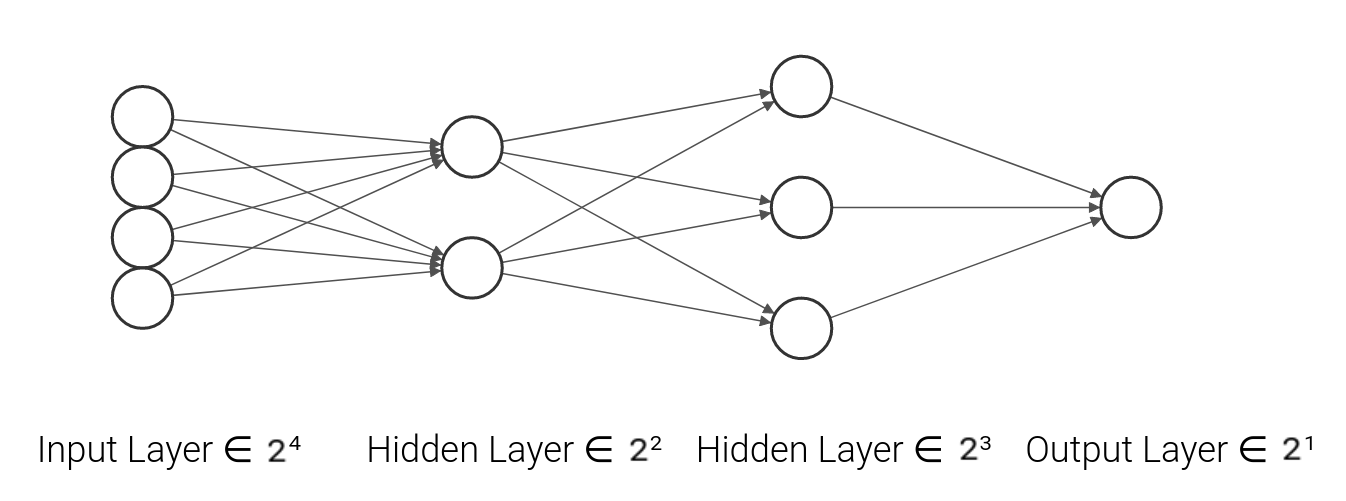
\includegraphics[width=0.75\textwidth]{capturas/esquemaMLPerceptron.png}}
    \caption{\textit{Perceptron} frente a \textit{Multilayer Perceptron}}
  \end{figure}


Y este fue precisamente el siguiente escalón a rebasar, superado ya en
la década de 1980, gracias a las \textit{Neuronas Sigmoides}
\textit{Perceptron}\textsuperscript{\cite{sancho}}, afines al
\textit{Perceptron} pero con la capacidad de trabajar con números reales.
La función de salida ahora sería una sigmoide, a la que deben su nombre y
convirtiéndose en la primera función de activación.

A partir de aquí y durante toda la década, comenzaron a aparecer todo tipo
de novedades que continúan vigentes: redes \textit{feedforward}, el algoritmo
\textit{backpropagation} o la \textit{Red Neuronal Convolucional}
(\textit{Convolutional Neural Network}, CNN)\textsuperscript{\cite{geo}}.
Las \textit{CNN} son especialmente convenientes para procesamiento de
imagen y vídeo, en general información espacial, aunque también se han
usado para tareas de procesamiento
de lenguaje natural. Esto es debido a que la información se divide en subcampos que sirven como
entrada a capas de procesamiento convolucional (ver Figura \ref{cnn}), encargadas de apreciar
las distintas carcterísticas que servirán para la clasificación de la
información de entrada.

\begin{figure}[h]
    \centering
    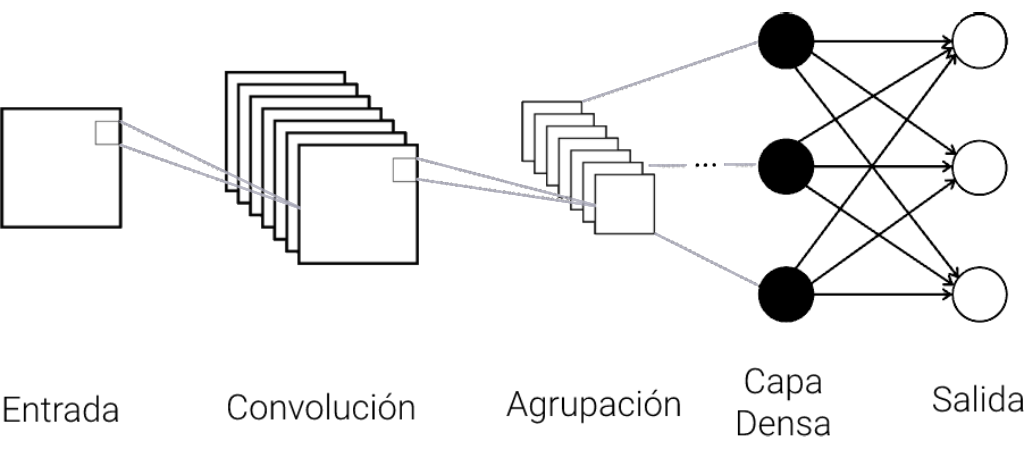
\includegraphics[width=0.69\textwidth]{capturas/CNN.png}\\[-0,20cm]
    \caption{Estructura simplificada de \textit{Red Neuronal Convolucional}\label{cnn}}
\end{figure}

Es llamativo ver cómo las \textit{CNN}, redes que mantienen su vigencia
pese a que su origen se remonta a poco antes de los 90. Pero la realidad es
que, si bien no lo parece, el campo de las redes neuronales lleva con nosotros
mucho tiempo y las \textit{CNN} no son el único ejemplo manifiesto.
Las \textit{Recurrent Neural Networks}, originadas en 1989, continúan en
uso para procesamiento de datos secuenciales como lo es por ejemplo el texto.

Fue en 2006 cuando \textit{Geoffrey Hinton et al} publicaron un famoso
paper\textsuperscript{\cite{hinton}} presentando una red neuronal profunda,
que entrenada, era capaz de reconocer dígitos. Acuñando como \textit{Deep Learning},
a la técnica del \textit{Machine Learning} (ya que se basa en el aprendizaje
automático), que usa como mecanismo de procesamiento redes neuronales profundas.
Se superaba entonces la barrera del entrenamiento de redes neuronales profundas,
barrera que había llevado a la comunidad a congelar el avance de esta técnica,
y que ahora elevaba al \textit{Deep Learning}
un nivel por encima del resto de técnicas del \textit{Machine Learning}.

El siguiente hito llegaría a mediados de los 2000 al poder trabajar
con redes neuronales profundas (\textit{Deep Learning}), gracias a la
introducción de pre-entrenamientos no supervisados para la asignación
de pesos previos al usual entrenamiento del modelo. Este avance fue
posible debido al desarrollo de la computación con GPUs.


El último acontecimiento o adición reseñable es el de las
\textit{Generative Adversarial Networks} (2014)
\textsuperscript{\cite{genAd}}, sujeto al empleo de dos
redes neuronales complementarias: una se denomina \textit{Generative network}
en calidad de modelo generador de muestras y otra \textit{Discriminative network}
que evalúa las muestras generadas por la anterior y por el dataset de entrenamiento,
es decir, recibe como entrada, la salida de la red anterior y del conjunto
de datos de entrenamiento. El proposito de esta simbiosis es que la red
generativa consiga reproducir muestras tan válidas como las de entrenamiento,
a partir del juicio de la red discriminativa.


De entonces hasta ahora, más que innovación, se han dado muchos avances
en términos de implementación, es habitual que cada cierto tiempo salga
una nueva aplicación revolucionaria o con mucho potencial que está basada
en redes neuronales. Y también es muy frecuente que gigantes tecnológicos
como por ejemplo \textit{Google} o \textit{Facebook} compren otros
proyectos basados en redes neuronales o directamente las empresas
que los llevan a cabo. Siendo una de las más destacables la compra de
\textit{DeepMind} por parte de \textit{Google} o la alianza entre
\textit{OpenIA} y \textit{Microsoft}.


Algunos ejemplos de estos proyectos son:
el tan sonado algoritmo de \textit{AlphaGo}\textsuperscript{\cite{alphago}}
de la empresa \textit{DeepMind},
capaz de vencer al campeón mundial del juego tablero \textit{Go}; el
proyecto \textit{DeepFace} de \textit{Facebook} para identificar y automatizar
el etiquetado de los usuarios en las imágenes; el \textit{AlphaFold2}
\textsuperscript{\cite{alphafold}} de
\textit{DeepMind}, capaz de predecir la estructura de las proteínas y que
ha sido revolucionario para la resolución del problema del plegamiento de
proteínas, lo que antes eran investigaciones del orden de 1 o 2 años, ahora
es computable en pocas horas; \textit{GPT-3}
\textsuperscript{\cite{openai}} de \textit{OpenIA},
un modelo de lenguaje cuya definición podría responder a \textit{chatbot},
es capaz de completar texto, responder preguntas o cualquier tarea que
implique interacción con texto; \textit{Copilot}\textsuperscript{\cite{ghcopilot}}
de \textit{OpenIA}
y \textit{Github, Microsoft}, un sistema construido sobre los cimientos de
\textit{GPT-3} capaz de sugerir código autogenerado
y comentarios analizando bien las directrices de un comentario o bien
directamente interpretando lo que el programador busca; \textit{Nerf}\textsuperscript{\cite{nerfs}}
de \textit{Nvidia}, capaz de generar composiciones 3D a partir de
imágenes fíjas; o por finalizar esta interminable lista de apasionantes
ejemplos, el reciente \textit{DALL.E}\textsuperscript{\cite{openai}} de \textit{OpenAI}, modelo generador
de imágenes a partir de una entrada de texto descriptora.

No se puede quedar sin mencionar las que han sido las dos últimas grandes
agitaciones del mundo de las redes neuronales y que están detrás de la
mayoría de los ejemplos anteriores: el \textit{Natural Language Processing}
y los \textit{Transformers}, aunque en realidad, van de la mano.
Van de la mano porque el \textit{Natural Language Processing}\textsuperscript{\cite{nlp}}
ya es
en sí mismo una revolución para el mundo de las redes neuronales, ya que
el procesamiento de lenguaje, dado que las redes interpretan información
numérica, siempre ha sido un desafío para el campo del \textit{Machine Learning};
y no ha sido hasta su llegada, que gracias a lo que propone (vectorización de
\textit{tokens}, que son los bloques de datos que se interpretan, ya sean
palabras o generalmente en la práctica, subpalabras), que las redes
no han empezado a operar de una forma realmente veraz con el lenguaje.
Sin embargo no solo ha sido una revolución en sí mismo, sino que ha
propiciado el nacimiento de otra como lo son los \textit{Transformers}\textsuperscript{\cite{transformers}},
que parten del progreso conseguido en las redes recurrentes o para ser más
precisos, de sus \textit{Mecanismos de Atención}\textsuperscript{\cite{aiayn}},
ya que es lo único que
mantienen respecto a los modelos recurrentes, es más, se alejan íntegramente
pasando a un procesamiento simultáneo y sustituyendo la ordenación recurrente
por la vectorización. Aunque pese a renunciar a la recurrencia, y es ahí donde
reside su potencial, continúan funcionando con información secuencial.

Esta mejora en la implementación y aparición de tantas aplicaciones
puede inferirse que se debe al aumento de la capacidad de cómputo de
las GPUs, la llegada de los \textit{Transformers},
la entrada de los mayores gigantes tecnológicos, pero sin
duda a la aparición de herramientas de alto nivel e infraestructuras
para el trabajo con redes neuronales como lo son \textit{Azure},
\textit{Aporia}, \textit{TensorFlow}, \textit{Keras}, \textit{SciKit-Learn},
etc.

\section{Microcontroladores}
Los microcontroladores son sistemas de dimensiones reducidas y bajo consumo,
destinados en su inicio al control de electrodomésticos, pero que a lo largo
del tiempo y sobre todo propiciado por la aparición del
\textit{Internet of things} (\textit{IoT}), y los avances en \textit{IA} han
supuesto un cambio en cómo se diseñan e implementan los nuevos dispositivos
electrónicos.

El primer microcontrolador fue desarrollado por \textit{Gary Boone} y
\textit{Michael Cochran} en 1971 y fue bautizado como
\textit{TSM 1000}\textsuperscript{\cite{mccon}}, albergando una arquitectura
\textit{Harvard} en un mismo circuito contando con el propio microprocesador,
memoria ROM, menos de 256 bytes de memoria RAM y el propio reloj del sistema.

Como respuesta, \textit{Intel} comercializó en 1977 su propio sistema para
aplicaciones de control, el \textit{Intel 8048}\textsuperscript{\cite{mcs48}},
que obtuvo gran popularidad y supuso un pequeño cambio en el paradigma de
ventas de \textit{Intel}.

Las memorias que montaban eran \textit{EPROM} en el caso de los microcontroladores
reprogramables y \textit{PROM} en el caso de los de bajo  presupuesto. Sin embargo esto
cambió con la llegada en 1993 de la \textit{EEPROM}, utilizada por primera vez
en el \textit{PIC16x64}\textsuperscript{\cite{mccon}} de \textit{Microchip} y que conllevó un gran avance
gracias a la agilización del proceso de creación de prototipos y su programación.

Poco después \textit{Atmel} implementaría por primera vez memoria \textit{flash}
en un microcontrolador y se usaría en el \textit{Intel 8051}, que trajo
ciertos cambios respecto a su predecesor, como pasar a arquitectura
\textit{Von Neumann} o la inclusión de
\textit{Universal Asynchronous Receiver-Transmitter}
(\textit{UART}) para el manejo de puertos y dispositivos serie. Además contaba
con múltiples compiladores de \textit{C} para su programación, alternativos
al lenguaje \textit{ensamblador}.

Gracias a la inclusión de estas dos últimas memorias en el diseño estandarizado de
los microcontroladores, el precio comenzó a ser cada vez más accesible.
También se inició la incorporación de periféricos complementarios para dotar
a los microcontroladores de más funcionalidad. Periféricos tales como generadores
\textit{PWM}, conversores analógicos A/D y D/A, relojes de tiempo real, etc.

Estos complementos lucen ahora arcaicos en comparación con los que se integran
en microcontroladores actuales: transceptores 802.15.4, bluetooh, wifi, cámaras,
micrófonos, y sensores de todo tipo como de presión, movimiento, orientación, color,
brillo, proximidad, humedad, etc. Todos estos acompañados de complejos microprocesadores
de 32 bits, cada vez más semejantes a las \textit{CPU}s de equipos de mayores
dimensiones. El progreso de los microprocesadores reducidos, ha sido propiciado
por el vasto crecimiento del mercado móvil en los últimos años. Y resultando
\textit{ARM}, al igual que para los smartphones, una excelente baza para la
complejidad que demandan los microcontroladores actuales.

Por un lado, su contenida complejidad frente a equipos de escritorio, hace que
económicamente su implementación sea muy viable, aunque esto mismo provoca
ciertos inconvenientes a la hora de su empleabilidad para \textit{IA}, mencionados
en la siguiente sección.


\section{Integración de redes neuronales en microcontroladores\label{integRNenμC}}
Algunos microcontroladores modernos dan soporte a herramientas para la \textit{IA},
como lo es la integración de redes neuronales;
sin embargo, el desarrollo de estas sigue siendo dependiente de la asistencia de un
PC. De igual forma este soporte a herramientas para la \textit{IA} es aun así
sorprendente viendo los resultados que se pueden obtener de su implementación y
siendo este proyecto muestra de ello.
Aunque en algunas ocasiones son necesarios ciertos arreglos dadas las carencias
de estos dispositivos, como en ciertos casos, la falta de \textit{FPU}s
(\textit{Floating-Point Unit}), suponiendo un obstáculo debido a que las redes
neuronales realizan su procesamiento en coma flotante.

Se precisa de equipos con mayores prestaciones para la
creación y entrenamiento de las redes neuronales que integrarán los microcontroladores,
ya que es un proceso complejo y costoso;
por suerte no es así para la ejecución, lo que los convierte en grandes candidatos
gracias al \textit{CloudML}, \textit{EdgeML} o \textit{TinyML}.

El \textit{CloudML}\textsuperscript{\cite{CloudMl}} es la técnica por la que, alojando redes neuronales profundas
en la nube, podemos integrar el uso de las mismas en \textit{TPU}s (Unidades de procesamiento
tensorial) y \textit{FPGA}s, entre otras. Esta alternativa presenta la capacidad
de emancipar el propio procesamiento de los algoritmos de \textit{Macine Learning}
fuera del propio dispositivo en el que se integra su implementación. Por otro lado,
supone contar con infraestructuras que den soporte a ello y el uso de herramientas
y entornos de pago, como entre otros el \textit{Google Cloud ML Engine}.

\textit{EdgeML}\textsuperscript{\cite{EdgeMl}} es una librería escrita en \textit{Python} propulsada por
\textit{GitHub, Microsoft} que mediante \textit{TensorFlow} (o alternativamente en
fase experimental \textit{Pytorch}), provee de distintas funciones enfocadas al
entrenamiento, evaluación y despliegue de algoritmos de
\textit{Machine Learning} para sistemas embebidos empleados para labores simples.
Por lo que es una elección perfecta para aquellos proyectos en los que se quiera
trabajar con \textit{Machine Learning} y utilizar herramientas de apoyo
\textit{open source}. Aunque cabe mencionar que, al tratarse de una herramienta
para \textit{Machine Learning} en general, las opciones dirigidas a
\textit{Deep Learning} no abundan.

\textit{Micro-Learn}\textsuperscript{\cite{microlearn}} es una librería para
\textit{python} que convierte modelos de \textit{machine learning} entrenados
con \textit{Scikit-Learn},
a código que virtualiza la ejecución del modelo en cualquier microcontrolador
en tiempo real.
Es relevante destacar que no existen demasiados proyectos, aunque a cambio
ofrece, en principio, soporte para cualquier microcontrolador \textit{arduino}.

También existen infinidad de destacables alternativas para \textit{FPGA}s como
\textit{Vitis-AI} o \textit{VTA}, entre otras, aunque no presentan soporte a
microcontroladores, por lo que quedan fuera de nuestro espectro de posibilidades.

Y finalmente, \textit{TinyML}\textsuperscript{\cite{tinyMl}} se define como el
campo que comprende a las tecnologías y aplicaciones relacionadas con el
\textit{Machine Learning} y que se fundamenta en la implementación de algoritmos
y software capaces de realizar análisis de datos de sensores en un hardware
muy limitado y de bajo consumo energético. Encontrando en esta alternativa,
numerosos proyectos que consultar, gran actividad de su comunidad y cuantiosa
documentación en forma de libros y publicaciones de usuarios.

\begin{comment}
En el campo del \textit{Deep Learning} integrado en sistemas empotrados, hay múltiples proyectos que
poder estudiar y observar previos a comenzar nuestro trabajo.\\\\
Disponemos, en el caso preciso de Arduino, aunque como sabemos no es el único fabricante de
este tipo de dispositivos; de una plataforma donde se exponen numerosos ejemplos de entusiastas
de Arduino que publican de forma abierta su código\cite{project-hub}. Y entre todos ellos, podemos encontrar
varios planteamientos haciendo uso de \textit{Machine Learning} como herramienta de procesamiento procesamiento.
\newline Estos proyectos suelen haberse diseñado para la placa con la que trabajaremos, ya que es no
hay plétora de dispositivos que posean capacidad de trabajar con TensorFlow.\\
La mayoría de los proyectos que podemos encontrar, son más demostraciones técnias y pequeñas
introducciones al trabajo con \textit{TensorFlow}, que proyectos con alguna finalidad. Pero aun así, me
han sido de enorme utilidad para entablar contacto con el entorno y dinámica de trabajo.\\
Hay uno de estos trabajos, o más que trabajos, desarrolladores, que ha sido un pilar para este
proyecto; se trata de \textit{Pete Warden}, probablemente la persona más ilustre en \textit{TensorFlow+Arduino}.
\textit{Pete Warden} es entre otros, el creador de uno de los libros que ha sido determinante para
documentarme y comenzar con TinyML: "\textit{TinyML: Machine Learning with TensorFlow Lite on
Arduino and Ultra-Low-Power Microcontrollers}"\cite{TinyML-PW}.\\
El \textit{magic\_wand}\cite{github-magicwand} de Arduino fue para mí la toma de contacto precedente a comenzar a realizar mi propio
código. Sin embargo fue la versión de \textit{Pete Warden}\cite{petewardenmw} la que ha servido como cimiento al desarrollo
del software que cargaré en la placa y en el que he terminado de comprender las dinámicas de trabajo
para TinyML.\\

Respecto al diseño y entrenamiento del modelo, no hay demasiados referentes.
Pero cabe destacar lo muy conveniente que es el libro "\textit{Hands-on Machine Learning
with Scikit-Learn, Keras, and TensorFlow}"\cite{Aurelien}. No solo estimable para TinyML, sino
para comprender muchos de los conceptos generales y bases teóricas y matemáticas
de \textit{TensorFlow}. Incluso como introducción a la práctica para crear tus primeros modelos,
ya que como se infiere del título, también se tratan herramientas de alto nivel que facilitan
la implementación de los modelos como lo son \textit{Scikit} o \textit{Keras}. Esta última
será esencial para nuestro planteamiento de modelo.
\end{comment}